\documentclass[12pt, a4paper]{article}

\usepackage{amsmath}
\usepackage{amsfonts}
\usepackage{amssymb}
\usepackage{graphicx}
\usepackage{float}
\usepackage{listings}
\usepackage{rotating}
\usepackage{tikz}
\usepackage{verbatim}
\pdfgentounicode=1
\pdfmapline{+cyberb@Unicode@  <cyberbit.ttf}

\begin{document}

\title{CloudGraph}
\author{P. Baillehache}
\date{\today}
\maketitle

\tableofcontents

\section*{Introduction}

CloudGraph is a C library of functions generating a 2D graphical representation of a graph based on the relations between its nodes. Two types of relation are considered: edges of the graph, and categories of nodes in the graph.\\

It also provides a front end which reads the graph definition from a text file or generate a random one, produces a TGA picture representing the network, and/or prints the nodes' 2D coordinates.\\

The representation of the graph has 2 modes: circular and linear. The representation of the links has 2 modes: straight line and curved line. Categories are represented by different color, and links between two categories have shading colors. Nodes and categories are also identified by labels which can be displayed.\\

\section{Input}

The description of the CloudGraph is given as input to the front end as a text file. The format of this text file is as follow:\\

\begin{scriptsize}
\begin{ttfamily}
\begin{lstlisting}
<number of category>
for each category: <id> <red> <green> <blue> <label> 
<number of node>
for each node: <id> <id of the category> <label>
<number of link>
for each link
<id first node> <id second node>
\end{lstlisting}
\end{ttfamily}
\end{scriptsize}

$<$id$>$ is an integer between 0 and the number of category/node minus one. $<$red/green/blue$>$ are integers between 0 and 255. $<$label$>$ is the displayed label, it cannot be empty.\\

\section{Interface}

\begin{scriptsize}
\begin{ttfamily}
\verbatiminput{../cloudgraph.h}
\end{ttfamily}
\end{scriptsize}

\section{Code}

\begin{scriptsize}
\begin{ttfamily}
\verbatiminput{../cloudgraph.c}
\end{ttfamily}
\end{scriptsize}

\section{Makefile}

\begin{scriptsize}
\begin{ttfamily}
\verbatiminput{../Makefile}
\end{ttfamily}
\end{scriptsize}

\section{Usage}

\begin{scriptsize}
\begin{ttfamily}
\verbatiminput{../main.c}
\end{ttfamily}
\end{scriptsize}

Output:\\

\begin{scriptsize}
\begin{ttfamily}
\begin{lstlisting}
main -print

Families:
#0 rgb(249,012,211) Family000
#1 rgb(110,015,053) Family001
Nodes:
#0 family(0) <0.000,18.000> Node000
#1 family(0) <0.000,54.000> Node001
#3 family(0) <0.000,90.000> Node003
#4 family(0) <0.000,126.000> Node004
#6 family(0) <0.000,162.000> Node006
#8 family(0) <0.000,198.000> Node008
#11 family(0) <0.000,234.000> Node011
#13 family(0) <0.000,270.000> Node013
#15 family(0) <0.000,306.000> Node015
#2 family(1) <0.000,342.000> Node002
#5 family(1) <0.000,378.000> Node005
#7 family(1) <0.000,414.000> Node007
#9 family(1) <0.000,450.000> Node009
#10 family(1) <0.000,486.000> Node010
#12 family(1) <0.000,522.000> Node012
#14 family(1) <0.000,558.000> Node014
Links:
000-006
001-007
002-013
003-005
004-010
005-010
007-013
009-015
011-012
\end{lstlisting}
\end{ttfamily}
\end{scriptsize}


\begin{center}
\begin{figure}[H]
\centering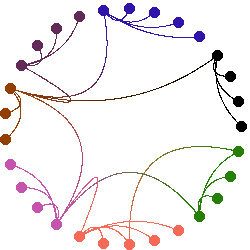
\includegraphics[width=5cm]{./cloud01.jpg}\\
\end{figure}
\end{center}
\begin{center}
\begin{figure}[H]
\centering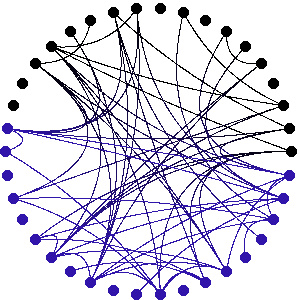
\includegraphics[width=5cm]{./cloud02.jpg}\\
\end{figure}
\end{center}
\begin{center}
\begin{figure}[H]
\centering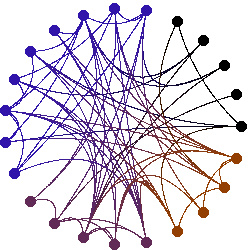
\includegraphics[width=5cm]{./cloud03.jpg}\\
\end{figure}
\end{center}
\begin{center}
\begin{figure}[H]
\centering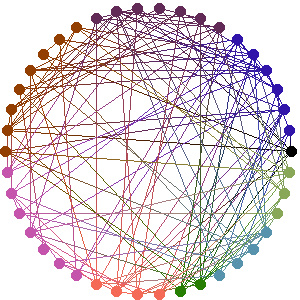
\includegraphics[width=5cm]{./cloud04.jpg}\\
\end{figure}
\end{center}
\begin{center}
\begin{figure}[H]
\centering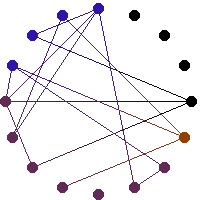
\includegraphics[width=5cm]{./cloud05.jpg}\\
\end{figure}
\end{center}
\begin{center}
\begin{figure}[H]
\centering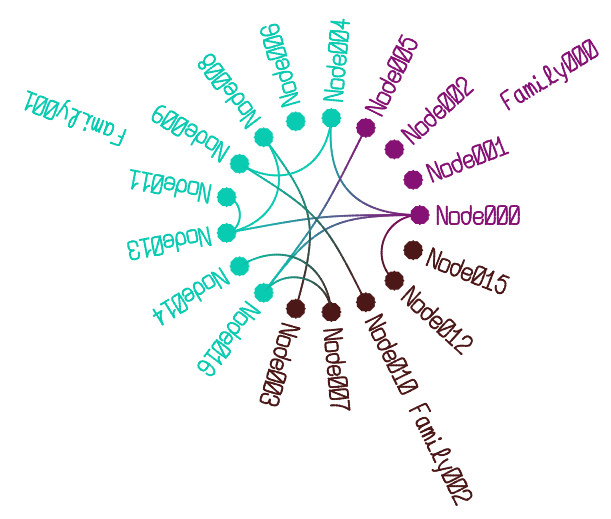
\includegraphics[width=5cm]{./cloud07.jpg}\\
\end{figure}
\end{center}
\begin{scriptsize}
\begin{ttfamily}
\begin{lstlisting}
main -file testCloud.txt -nodeLabel -familyLabel
\end{lstlisting}
\end{ttfamily}
\end{scriptsize}
\begin{center}
\begin{figure}[H]
\centering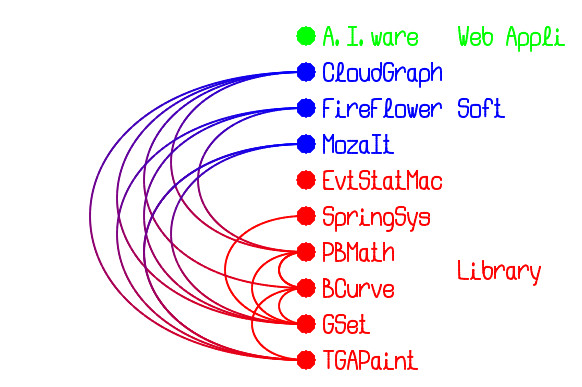
\includegraphics[width=5cm]{./cloud06.jpg}\\
\end{figure}
\end{center}
\begin{scriptsize}
\begin{ttfamily}
\begin{lstlisting}
testCloud.txt :

3
0 255 0 0 Library 
1 0 0 255 Soft 
2 0 255 0 Web Appli
10
0 0 TGAPaint
1 0 GSet
2 1 MozaIt
3 1 FireFlower
4 0 BCurve
5 0 PBMath
6 0 SpringSys
7 0 EvtStatMac
8 2 A.I.ware
9 1 CloudGraph
16
4 5
4 1
5 1
5 4
6 1
0 4
9 1
9 5
9 4
9 0
3 1
3 5
3 0
2 1
2 0
\end{lstlisting}
\end{ttfamily}
\end{scriptsize}

\end{document}


